\section{Tuning Systems in Music}

\subsection{Frequency and Musical Notes}

In this section, we will only consider tones which correspond to periodic pressure waves. Their periodicity means that we can associate them with a certain frequency. Period notably doesn't mean that they are perfect sine waves as we have considered before, but rather an arbitrary periodic function. With the audible range going spanning from 20 Hz to 20.000 Hz, the question is now what kinds of frequencies we want to consider.

If you picture the keyboard of a piano with its discrete white and black keys, it is quite clear to see that (Western) music only deals with a handful of discrete frequencies. There is --- apart from esthetic ones --- no reason not to use the frequencies say, between D and D flat. If you have a string instrument, you can quite easily play at such a frequency by just putting your finger between the position for D flat and D . But now if you try to play it in combination with, let's say, G, it would sound somewhat ``off''. To some degree, it is still a matter of taste, but the music community has collectively agreed to use only a certain set of frequencies that they find most pleasant sounding. We call these sets \textbf{musical scales}. Since they are a matter of taste and convention, different cultures have developed different musical scales. For the moment, we'll focus on the ones that are most present in Western music. 

Before one can build a house, one must lay a foundation. In the case of music, we must choose one frequency that we want to start with, and from it we'll construct the rest.

A commonly used reference frequency in Western music is the A above the middle C. Its frequency is given by 
\begin{equation}
    f_A = 440 \,\text{Hz}.
\end{equation}

In the past, people have used a lower frequency for the A. It is thought that in Bach's times, the value might have been as low as $415$ Hz! This doesn't make Bach's music by any means unplayable in our modern times, though, since it turns out that \textbf{music is much less about absolute frequencies and all about ratios}.

\subsection{Octaves}

The most important ratio in music is 1:2, which we call an octave. 
For example, to obtain the frequency of A', the note one octave above the A above the middle C, we only have to double the frequency, so
\begin{align}
    f_{\text{octave}} &= 2 \cdot f \\
    f_{A'} = 2 \cdot f_A &= 880\, \text{Hz}.
\end{align}

One reason we care about octaves is that notes that are an octave apart like A and A' sound similar, and make a pleasant sound when combined. It therefore makes sense that given a note in a scale, the note an octave higher and lower should be also in the musical scale. (In fact, any number of octaves higher and lower should be in the scale.)

\textit{Question: What is the frequency of the note one octave lower than A?}

\subsection{Intervals}

With the frequency ratio for the octave fixed, we're left to determine the rest of the frequency ratios. The difference in pitch between two notes is called an \textbf{interval}. The size of an interval directly corresponds to a ratio in frequencies. For example, as we've seen before, an octave always corresponds to a ration of 2:1. 
Going up one key on the keyboards corresponds to one semitone step. There are twelve semitone steps in an octave. We now define:
\begin{itemize}
    \item \textbf{minor second} = one semitone step
    \item \textbf{major second} = two semitone steps
    \item \textbf{minor third} = three semitone steps
    \item \textbf{major third} = four semitone steps
    \item \textbf{perfect forth} = five semitone steps 
    \item \textbf{perfect fifth} = \textbf{seven} semitone steps 
    \item \textbf{minor sixth} = eight semitone steps 
    \item \textbf{major sixth} = nine semitone steps 
    \item \textbf{minor seventh} = ten semitone steps 
    \item \textbf{major seventh} = eleven semitone steps 
    \item \textbf{octave} = twelve semitone steps
\end{itemize}

The intervals are also shown in Fig. \ref{fig:intervalle} on a piano keyboard. In case you're not familiar with piano keyboards, the keys are labeled Fig. \ref{fig:piano_keyboard}. 

\begin{figure}[!htb]
    \centering
    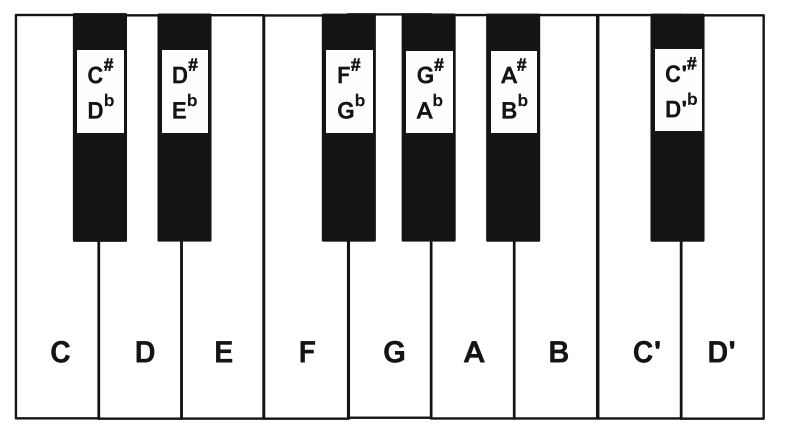
\includegraphics[width = 0.6 \textwidth]{Bilder/piano_keyboard.png}
    \caption{Keyboard of a piano with labeled notes}
    \label{fig:piano_keyboard}
    % Quelle : Physics of sound and color fig 12.3
\end{figure}


\begin{figure}[!htb]
    \centering
    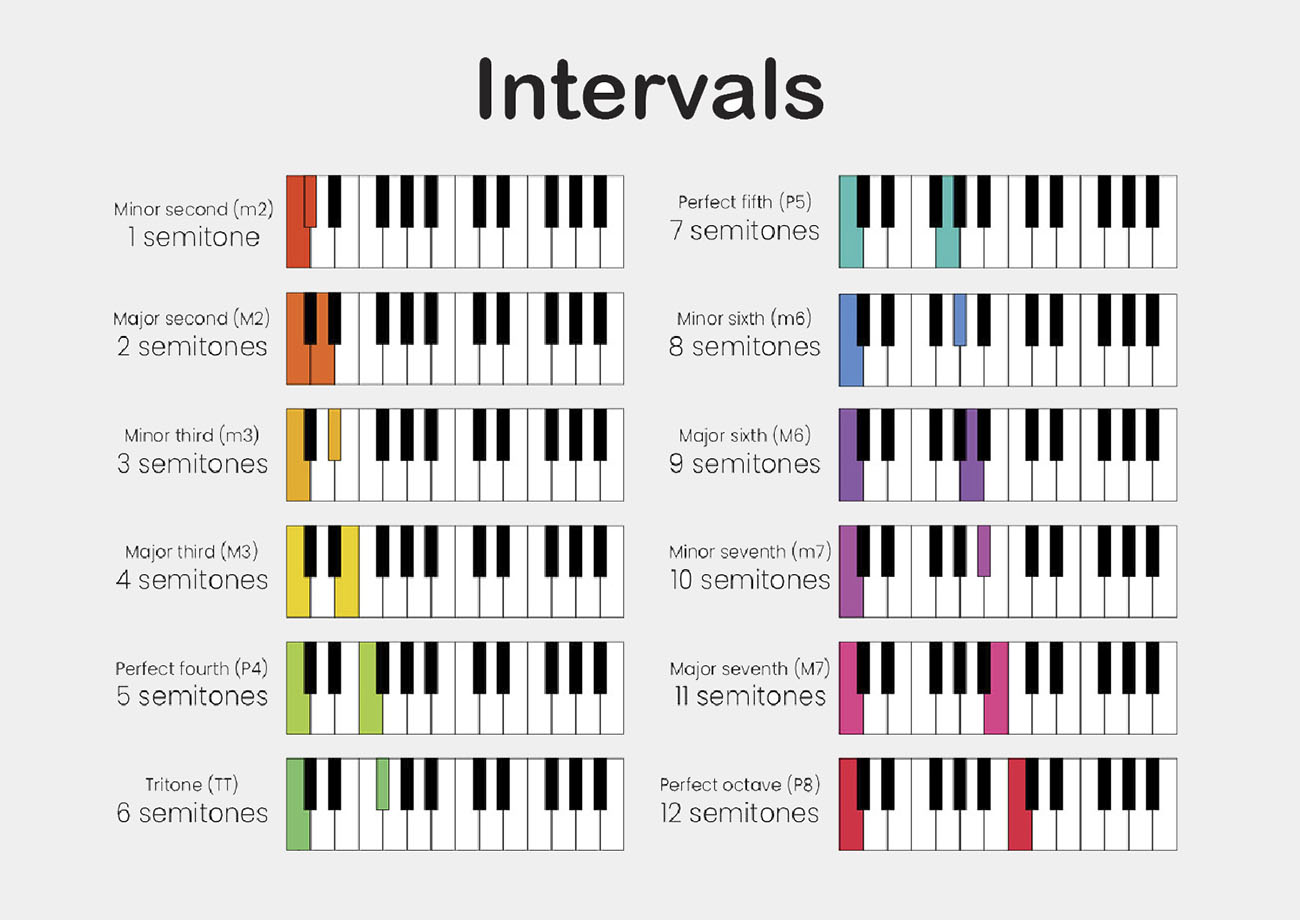
\includegraphics[width = 0.6 \textwidth]{Bilder/intervalle.jpg}
    \caption{Musical intervals on a piano keyboard}
    \label{fig:intervalle}
    % Quelle : https://woodandfirestudio.com/wp-content/uploads/2023/07/intervalleen.jpg
\end{figure}

Now that we can talk about intervals in precise language, the question is what frequency ratios we want to assign to the different intervals. This choice determines the tuning. We will talk here about three kinds of tuning:  Pythagorean tuning, Just tuning and Equal Temperament.

\subsection{Pythagorean tuning}
Pythagorean tuning treats the fifth as the most important interval (apart from the octave) with a fixed ratio of $3:2$, and deduces from it all other intervals. 

Why $3:2$? Let's say for a moment, that our two frequencies are $f_1 = 400$ Hz and $f_2 = 600$ Hz, and that we're playing them on, say, two strings. The harmonics of $f_1$ are integer multiples of $f_1$, so 400 Hz, 800 Hz, 1200 Hz, ... and for $f_2$, we have 600 Hz, 1200 Hz, 1800 Hz, ... 
Note how the frequency 1200 Hz shows up in both sequences. This leads to a resonance between the two strings, enriching the overall sound, and making it sound pleasant. For this reason, low integer ratios like $3:2$ are said to sound \textbf{consonant}. On the other hand, high integer ratios tend to sound \textbf{dissonant}. To test this, try playing C and G and then C and C sharp on the piano! The first interval is a fifth, which sounds consonant, the second interval is a minor second and sounds dissonant. 

Let's now ascend in steps of fifths an use the ratio $3:2$ to determine the frequencies. We'll use $C_4$ (the middle C) as our reference frequency. 

\[
\begin{array}{c@{\;\rightarrow\;}c@{\;\rightarrow\;}c@{\;\rightarrow\;}c@{\;\rightarrow\;}c@{\;\rightarrow\;}c@{\;\rightarrow\;}c}
F_3 & C_4 & G_4 & D_5 & A_5 & E_6 & B_6 \\
2/3 & 1 & 3/2 & (3/2)^2 & (3/2)^3 & (3/2)^4 & (3/2)^5
\end{array}
\]

Now, we can ascend and descend by an octave by using the ratio $2:1$.

\[
\begin{array}{c@{\;\rightarrow\;}c@{\;\rightarrow\;}c@{\;\rightarrow\;}c@{\;\rightarrow\;}c@{\;\rightarrow\;}c@{\;\rightarrow\;}c}
F_4 & C_4 & G_4 & D_4 & A_4 & E_4 & B_4 \\
4/3 & 1 & 3/2 & (3/2)^2 \cdot 1/2 & (3/2)^3 \cdot 1/2 & (3/2)^4 \cdot 1/4& (3/2)^5  \cdot 1/4 \\
4/3& 1& 3/2 & 9/8 & 27/16 & 81/64 & 243/128
\end{array} \\
\]

So, by reordering, we have 

\[
\begin{array}{c@{\;\;}c@{\;\;}c@{\;\;}c@{\;\;}c@{\;\;}c@{\;\;}c}
C_4 & D_4 & E_4 & F_4 & G_4 & A_4 & B_4 \\
1 & 9/8 & 81/64 & 4/3 & 3/2 & 27/16 & 242/128
\end{array} \\
\]
From this we can already tell that the forth from $C_4$ to $F_4$ will sound consonant in Pythagorean tuning, whereas the major third $C_4 - E_4$ will sound relatively dissonant because of the large integer ratio. Traditionally, we want the major third to sound consonant. This problem will be addressed by just tuning.

The other notes can be obtained in a similar manner. If it interests you, you can find them on Wikipedia, under Pythagorean tuning.

\textit{Question: What is the frequency ratio for the two semitones C-D? What about D-F, F-G and G-A?}

\textbf{Answer:} $f_D/f_C = 9/8$, $f_F/f_D = f_F/f_C \cdot f_C/f_D = 4/3 \cdot 8/9 = 32 / 27$, $f_G/f_F = 9/8$, $f_A/f_G = 9/8$. In particular, an interval of two semitones doesn't always correspond to the same frequency ratio!


\subsection{Just tuning}


\subsection{Equal Temperament}

In modern music, the octave is divided into 12 equal steps.

Each step corresponds to multiplying the frequency by the same factor.

\begin{equation}
    f_n = f_0 \cdot 2^{\frac{n}{12}}
\end{equation}

\paragraph{Intuitive Explanation:}
\begin{itemize}
    \item Instead of using simple fractions, we divide the octave evenly
    \item Each step sounds similar in size
\end{itemize}

\paragraph{Why is this useful?}
It allows us to play in all keys without retuning the instrument.

\paragraph{But:}
The intervals are not perfectly ``pure'' anymore — this is a compromise.
